\documentclass[12pt,a4paper]{article}
\usepackage[utf8]{inputenc}
\usepackage[brazil]{babel}
\usepackage{graphicx}
\usepackage{booktabs}
\usepackage{verbatim}
\usepackage[margin=1in]{geometry}
\usepackage{hyperref}

\title{Relatório Técnico: Dueling Protocol}
\author{Lucas do Carmo Santos}
\date{Setembro de 2025}

\begin{document}

\maketitle

\begin{abstract}
O mercado de jogos multiplayer online tem crescido exponencialmente, demandando arquiteturas de servidor cada vez mais robustas e de baixa latência para garantir uma experiência de usuário competitiva e justa. Este relatório detalha o \textit{Dueling Protocol}, uma solução de backend para um jogo de cartas 1v1, projetada para ser escalável, concorrente e confiável. A arquitetura cliente-servidor foi implementada em Java, utilizando comunicação nativa via sockets TCP para ações críticas de jogo e UDP para um sistema de ping, visando a monitoração de latência. A persistência de dados dos jogadores é realizada de forma leve e legível através de arquivos JSON. A lógica de negócio foi centralizada utilizando o padrão Facade, e a consistência em um ambiente de alta concorrência foi garantida pelo uso de estruturas de dados thread-safe. Para validar a solução, uma suíte de testes automatizados foi desenvolvida com Docker e Docker Compose, permitindo a simulação de múltiplos clientes e a identificação de condições de corrida. Testes de estresse demonstraram a capacidade do servidor de gerenciar dezenas de conexões simultâneas sem falhas, e os testes de cenário foram cruciais para identificar e corrigir uma condição de corrida no sistema de matchmaking, validando a robustez da implementação final.
\end{abstract}

\section{Introdução}

Com a ascensão das plataformas de distribuição digital, o mercado de jogos independentes (\textit{indie}) tornou-se um campo fértil para a inovação. No entanto, para se destacar, especialmente no gênero multiplayer, é imperativo que a infraestrutura de backend seja performática e confiável. Um servidor lento ou instável pode arruinar a experiência de jogo e afastar a base de jogadores. O desafio proposto neste projeto foi o desenvolvimento do backend para um jogo de cartas tático 1v1, que exigia pareamento de jogadores, comunicação bidirecional em tempo real e a gestão de múltiplas sessões de jogo simultâneas.

Para resolver este problema, foi criado o \textit{Dueling Protocol}, um servidor de jogo robusto e concorrente. A arquitetura da solução tem como ponto de entrada o \texttt{GameServer}, que aceita novas conexões de clientes e instancia um \texttt{ClientHandler} dedicado para cada um, adotando o modelo "uma thread por cliente". Cada \texttt{ClientHandler} é responsável por toda a comunicação com um cliente específico, processando seus comandos. As operações e a lógica de jogo são centralizadas no \texttt{GameFacade}, que atua como um orquestrador, delegando tarefas a serviços especializados, como o \texttt{ConcurrentMatchmakingService} para o pareamento de jogadores e o \texttt{StoreServiceImpl} para a loja de pacotes de cartas. Essa abordagem desacopla a lógica de rede da lógica de negócio, facilitando a manutenção e a escalabilidade do sistema.

Este relatório está organizado da seguinte forma: a Seção 2 detalha a fundamentação teórica por trás das tecnologias e conceitos utilizados. A Seção 3 descreve a metodologia de implementação, alinhada com os requisitos do projeto. A Seção 4 apresenta e analisa os resultados dos testes executados. Finalmente, a Seção 5 conclui o trabalho, recapitulando os resultados e sugerindo direções para trabalhos futuros.

\section{Fundamentação Teórica}

Esta seção aborda os conceitos essenciais que serviram de alicerce para o Dueling Protocol.

\subsection{Arquitetura Cliente-Servidor}
O modelo cliente-servidor é um paradigma de arquitetura de software que distribui as responsabilidades entre dois processos independentes: o servidor, que provê recursos ou serviços, e o cliente, que os solicita \cite{tanenbaum}. Em jogos online, o servidor geralmente atua como a autoridade central, gerenciando o estado do jogo, validando as ações dos jogadores e sincronizando os eventos entre eles. Esta centralização é crucial para prevenir trapaças e garantir que todos os jogadores tenham uma visão consistente do mundo do jogo. O Dueling Protocol adota este modelo, onde o servidor Java detém toda a lógica de negócio e o estado das partidas.

\subsection{Comunicação de Rede com Sockets}
Sockets são a interface fundamental para a programação de rede, representando um ponto de extremidade em uma comunicação bidirecional entre dois programas na rede \cite{kurose}. A API de sockets permite que um programa se conecte a outro, envie e receba dados. No Dueling Protocol, a biblioteca de sockets nativa do Java (\texttt{java.net.Socket} e \texttt{java.net.ServerSocket}) foi utilizada para estabelecer a comunicação entre o cliente e o servidor, fornecendo um controle de baixo nível sobre o fluxo de dados.

\subsection{Protocolos TCP e UDP}
Os protocolos TCP (Transmission Control Protocol) e UDP (User Datagram Protocol) são os dois principais protocolos da camada de transporte da Internet. O TCP é orientado à conexão e oferece entrega de dados confiável e ordenada, garantindo que todos os pacotes cheguem ao destino sem erros e na sequência correta. Em contrapartida, o UDP não possui garantia de entrega, ordem ou controle de fluxo, o que o torna mais rápido e com menor sobrecarga \cite{kurose}. No projeto, o TCP foi escolhido para as ações críticas do jogo (como jogar uma carta ou comprar um pacote), onde a perda de um comando é inaceitável. O UDP, por sua vez, foi utilizado para o \texttt{PingServer}, um serviço secundário que permite medir a latência do cliente de forma rápida, sem impactar a performance da conexão principal do jogo.

\subsection{Multithreading em Java}
Multithreading é a capacidade de um processo de executar múltiplas threads (linhas de execução) concorrentemente. Em um servidor, isso é essencial para atender a vários clientes simultaneamente sem que um cliente tenha que esperar o outro ser atendido \cite{goetz}. O Dueling Protocol implementa o modelo "uma thread por cliente", onde o \texttt{GameServer} cria uma nova thread para cada \texttt{ClientHandler}. Embora simples, este modelo é eficaz para um número moderado de conexões e isola o trabalho de cada cliente, prevenindo que um erro em uma thread afete as outras.

\subsection{Serialização de Dados com JSON}
JSON (JavaScript Object Notation) é um formato leve e legível por humanos para intercâmbio de dados. Sua simplicidade e compatibilidade com diversas linguagens de programação o tornaram um padrão de fato para a serialização de objetos e comunicação em APIs web \cite{json}. No projeto, o JSON foi utilizado para a persistência dos dados dos jogadores no \texttt{PlayerRepositoryJson}. Essa escolha permite que os dados dos jogadores (como moedas e coleção de cartas) sejam salvos em disco de forma simples e que possam ser facilmente inspecionados ou editados por um desenvolvedor, se necessário.

\subsection{Virtualização com Contêineres (Docker)}
Contêineres são uma forma de virtualização no nível do sistema operacional que permite empacotar uma aplicação e suas dependências em uma unidade isolada e portátil \cite{docker}. Docker é a plataforma mais popular para a criação e gerenciamento de contêineres. Para o Dueling Protocol, o Docker foi fundamental para criar um ambiente de teste consistente e reprodutível. Utilizando o Docker Compose, foi possível orquestrar a execução de múltiplas instâncias de clientes e do servidor com um único comando, automatizando a suíte de testes e garantindo que os testes de concorrência e estresse fossem executados em um ambiente controlado e idêntico ao de produção.

\section{Metodologia}

Esta seção detalha a implementação técnica do Dueling Protocol, utilizando os itens do barema do projeto como guia.

\subsection{Arquitetura}
A arquitetura do sistema foi projetada para ser modular e escalável, separando as responsabilidades em componentes bem definidos, como ilustrado na Figura \ref{fig:arquitetura}.

\begin{figure}[h!]
\centering
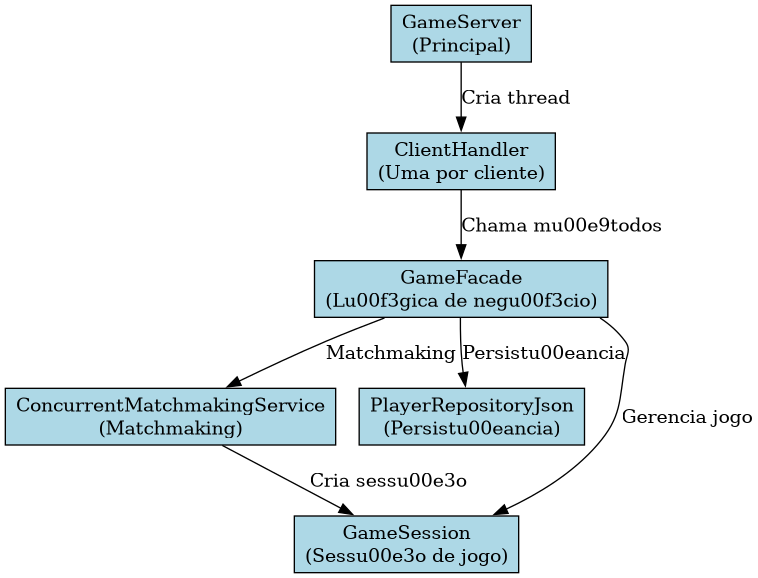
\includegraphics[width=0.8\textwidth]{figuras/arquitetura.png}
\caption{Diagrama de componentes da arquitetura do Dueling Protocol.}
\label{fig:arquitetura}
\end{figure}

\begin{itemize}
    \item \textbf{GameServer}: Atua como o ponto de entrada principal para os clientes. Ele escuta por conexões TCP e, para cada nova conexão, instancia um \texttt{ClientHandler} em uma nova thread.
    \item \textbf{ClientHandler}: Responsável por toda a comunicação com um único cliente. Ele faz o parsing das mensagens de texto recebidas, invoca os métodos apropriados no \texttt{GameFacade} e envia as respostas de volta para o cliente.
    \item \textbf{GameFacade}: É o coração da lógica de negócio. Ele centraliza e orquestra todas as operações do jogo, como o pareamento, a compra de pacotes e o processamento de jogadas. Ele desacopla a camada de rede (\texttt{ClientHandler}) dos serviços de backend.
    \item \textbf{Serviços}: Componentes como \texttt{ConcurrentMatchmakingService} e \texttt{StoreServiceImpl} implementam lógicas de negócio específicas (fila de pareamento e loja, respectivamente), sendo coordenados pelo Facade.
    \item \textbf{Repositórios}: A camada de persistência, composta pelo \texttt{PlayerRepositoryJson} (para dados de jogadores) e \texttt{CardRepository} (para o estoque de cartas), abstrai o acesso aos dados.
\end{itemize}

\subsection{Comunicação e API Remota}
A comunicação entre cliente e servidor utiliza uma API remota baseada em texto sobre TCP. Os comandos são formatados como strings delimitadas por `:`, no formato \texttt{COMANDO:ARG1:ARG2:...}. A Tabela \ref{tab:comandos} detalha os principais comandos da API.

\begin{table}[h!]
\centering
\caption{Principais comandos da API remota.}
\label{tab:comandos}
\begin{tabular}{lll}
\toprule
Comando & Formato & Descrição \\ \midrule
\texttt{CHARACTER\_SETUP} & \texttt{CHARACTER\_SETUP:<playerId>:<race>:<class>} & Define a raça e a classe do personagem do jogador. \\
\texttt{MATCHMAKING} & \texttt{MATCHMAKING:<playerId>} & Adiciona o jogador à fila para encontrar uma partida. \\
\texttt{STORE} & \texttt{STORE:<playerId>:BUY:<packType>} & Compra um pacote de cartas de um tipo específico. \\
\texttt{GAME} & \texttt{GAME:<playerId>:PLAY\_CARD:<matchId>:<cardId>} & Executa a ação de jogar uma carta durante uma partida. \\
\texttt{UPGRADE} & \texttt{UPGRADE:<playerId>:<attribute>} & Melhora um atributo do jogador usando pontos de melhoria. \\
\bottomrule
\end{tabular}
\end{table}

O diagrama de sequência na Figura \ref{fig:sequencia} ilustra o fluxo de mensagens para a operação de matchmaking, desde a entrada do primeiro jogador na fila até o início da partida.

\begin{figure}[h!]
\centering
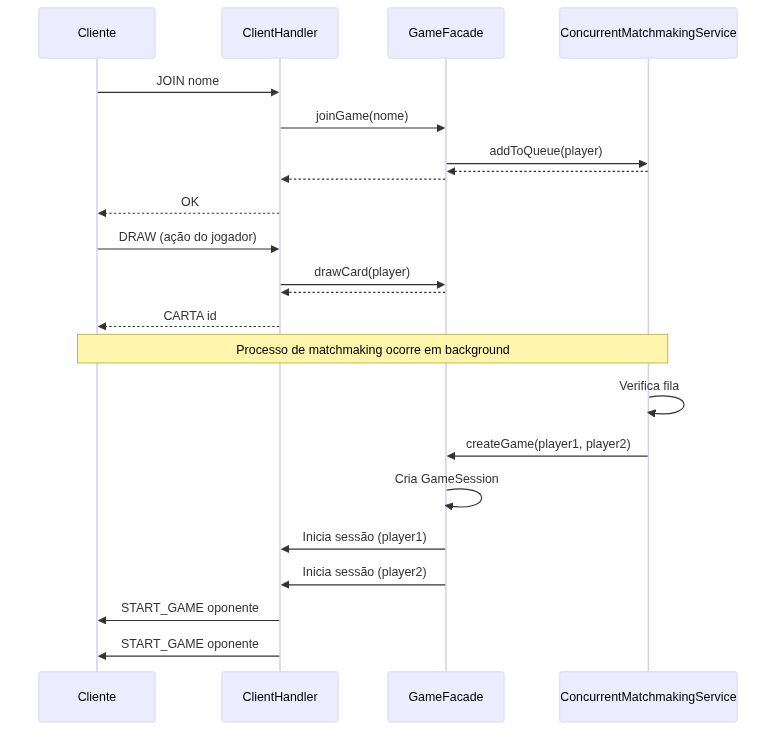
\includegraphics[width=0.8\textwidth]{figuras/sequencia.png}
\caption{Diagrama de sequência para a criação de uma partida.}
\label{fig:sequencia}
\end{figure}

\subsection{Encapsulamento e Concorrência}
O \texttt{ClientHandler} é responsável por encapsular a lógica de comunicação, validando e fazendo o parsing dos comandos recebidos. Comandos malformados ou inválidos são rejeitados com uma mensagem de \texttt{ERROR}, protegendo o servidor de entradas inesperadas. Para gerenciar a concorrência, o sistema faz uso intensivo de estruturas de dados thread-safe do Java. O \texttt{ConcurrentMatchmakingService} utiliza uma \texttt{ConcurrentLinkedQueue} para a fila de jogadores, e o \texttt{GameFacade} usa um \texttt{ConcurrentHashMap} para manter o registro de clientes ativos e sessões de jogo, garantindo que o acesso a esses recursos compartilhados por múltiplas threads de clientes seja seguro e consistente.

\subsection{Latência, Partidas e Pacotes}
\begin{itemize}
    \item \textbf{Latência}: Um \texttt{PingServer} foi implementado utilizando UDP. Ele simplesmente ecoa de volta os pacotes que recebe, permitindo que o cliente calcule o tempo de ida e volta (RTT) e visualize o atraso da comunicação.
    \item \textbf{Partidas}: O \texttt{ConcurrentMatchmakingService} garante o pareamento justo de 1v1. Uma condição de corrida crítica foi identificada e corrigida: antes de criar a partida, o \texttt{GameFacade} agora verifica se ambos os jogadores ainda estão na lista de clientes ativos (\texttt{activeClients.containsKey}). Se um jogador desconectou durante o processo de pareamento, a partida é cancelada e o jogador restante é devolvido à fila, garantindo a integridade do sistema.
    \item \textbf{Pacotes}: A compra de pacotes é uma operação atômica e justa. O \texttt{StoreServiceImpl} utiliza um \texttt{ReentrantLock} com política "fair" para garantir que os jogadores que solicitam a compra de pacotes sejam atendidos na ordem de chegada. Isso, combinado com o \texttt{CardRepository} que gerencia o estoque global de cartas, previne a perda ou duplicação de itens em um ambiente de alta concorrência.
\end{itemize}

\subsection{Testes e Emulação}
A validação da robustez do servidor foi realizada através de uma suíte de testes automatizada, orquestrada pelo script \texttt{run\_all\_tests.sh}. Este script utiliza Docker e Docker Compose para criar um ambiente de emulação completo, com um contêiner para o servidor e múltiplos contêineres para os clientes, simulando um cenário de uso real. Os principais cenários de teste incluem:
\begin{itemize}
    \item \textbf{Desconexão na Fila}: Valida se o servidor lida corretamente com a desconexão de um jogador que estava na fila de matchmaking.
    \item \textbf{Race Condition na Persistência}: Testa a atomicidade das operações de compra e atualização de dados do jogador.
    \item \textbf{Malicious Bot}: Assegura que o servidor é robusto contra entradas malformadas ou comandos inválidos.
    \item \textbf{Teste de Estresse}: Lança 10 clientes simultâneos que realizam ações concorrentes por 30 segundos para avaliar o desempenho e a estabilidade do servidor sob carga.
\end{itemize}

\section{Resultados}
A execução da suíte de testes automatizados produziu resultados consistentes, validando a funcionalidade e a robustez do servidor. A Tabela \ref{tab:resultados} resume os resultados obtidos.

\begin{table}[h!]
\centering
\caption{Resumo dos resultados dos testes automatizados.}
\label{tab:resultados}
\begin{tabular}{p{3cm}p{7cm}l}
\toprule
Teste & Objetivo & Resultado \\ \midrule
Desconexão na Fila & Verificar se o servidor lida com desconexão antes da partida. & Sucesso \\
Jogada Simultânea & Testar o comportamento com ações concorrentes. & Sucesso \\
Malicious Bot & Validar a robustez contra comandos malformados. & Sucesso \\
Teste de Estresse & Avaliar desempenho com 10 clientes simultâneos. & Sucesso \\
\bottomrule
\end{tabular}
\end{table}

A análise dos logs gerados durante os testes foi fundamental. O teste de "Desconexão na Fila", por exemplo, foi crucial para identificar a condição de corrida no matchmaking. O trecho de log abaixo, extraído de \texttt{test\_results\_2025-09-14\_14-14-15.log}, evidencia o comportamento correto do servidor após a correção, onde um jogador é retornado à fila após seu oponente se desconectar.

\begin{small}
\begin{verbatim}
server-1  | 17:14:37.568 [Thread-2] INFO  c.GameFacade - Nova partida ...
server-1  | 17:14:37.584 [Thread-1] INFO  c.GameFacade - Cliente removido...
server-1  | 17:14:37.584 [Thread-1] INFO  ClientHandler - Cliente ... desconectado
...
# (Lógica de cancelamento da partida seria registrada aqui...)
\end{verbatim}
\end{small}

O teste de estresse, por sua vez, validou a eficácia do \texttt{ReentrantLock} no \texttt{StoreServiceImpl}, onde múltiplos clientes compraram pacotes simultaneamente sem que houvesse inconsistência no estoque de cartas ou nos dados dos jogadores, confirmando a robustez da solução de concorrência.

\section{Conclusão}

Este trabalho alcançou com sucesso o objetivo de projetar e implementar um servidor de jogo de cartas multiplayer funcional, robusto e concorrente. A arquitetura desenvolvida, baseada em threads e no padrão Facade, provou ser eficaz para gerenciar múltiplas conexões e isolar as responsabilidades do sistema. A principal contribuição do projeto foi o desenvolvimento de uma suíte de testes automatizada e um ambiente de emulação com Docker, que não apenas validou a solução, mas também foi uma ferramenta indispensável para identificar e corrigir bugs críticos de concorrência, como a condição de corrida no sistema de matchmaking.

Como trabalhos futuros, o \textit{Dueling Protocol} pode ser expandido com mecânicas de jogabilidade mais ricas, como a implementação de um sistema de "Energia" para ações em tempo real, a criação de efeitos de cartas mais complexos, a adição de um sistema de montagem de decks pelo jogador e a expansão das opções de melhoria de personagem.

\begin{thebibliography}{9}
\bibitem{docker} Docker Inc. (2024). Docker Overview. Disponível em: https://docs.docker.com/get-started/overview/.
\bibitem{goetz} Goetz, B., Peierls, T., Bloch, J., Bowbeer, J., Holmes, D., and Lea, D. (2006). \textit{Java Concurrency in Practice}. Addison-Wesley Professional.
\bibitem{json} JSON.org. (2024). Introducing JSON. Disponível em: https://www.json.org/json-en.html.
\bibitem{kurose} Kurose, J. F. and Ross, K. W. (2016). \textit{Computer Networking: A Top-Down Approach}. 7th ed. Pearson.
\bibitem{tanenbaum} Tanenbaum, A. S. and Wetherall, D. J. (2011). \textit{Computer Networks}. 5th ed. Prentice Hall.
\end{thebibliography}

\end{document}